\section{Study 2 - Designing A COPD Telehealth System}     
In the following we describe how we redesigned the system to support the COPD patients in collecting and reflecting on self-tracked data and evaluated the re-design. 

\subsection{Methodological Considerations}
Initially, we planned to conduct co-designing activities with the COPD patients to meet their user needs. However, Das et al. found that co-design sessions with COPD patients using generative tools and techniques (e.g. post-it notes and sketching activities) is resource demanding for patients due to their health condition \cite{Das}. Some patients were not even able to participate in other activities than keeping a conversation. In Study 1, we similarly experienced that the COPD patients were physically limited (e.g. in terms of moving from one place to another) and within an hour of interview experienced breathing difficulties several times, demanding a slow pace and long pauses. Drawing from Das et al.'s experiences and our own experiences from Study 1, we decided not to conduct co-designing activities as initially planned. 

We made a conscious plan to conduct individual sessions, where patients were only expected to either talk or interact with a prototype. To further reduce time and effort required by patients in the sessions, patients completed workbook assignments beforehand, allowing them to prepare for the discussion on, how our proposals foster reflection during collection and review of data. In the following, we describe the workbook and prototype design.

\subsection{Workbook Design}
Workbooks assignments aimed at getting insight into, how the system can support patients in collecting and reflecting on data. Study 1 showed that patients were unsure, whether they were collecting data under the right conditions. We asked them to annotate, if they had reflected on context-relevant variables provided in the workbook to get further insight into, how patients reflect on conditions relevant for the validity and reliability of their measures. For dyspnea measures, context-relevant variables could be e.g. weather, mood, smoking or physical activity. Patients commented on it as free text annotation one day and mark it in checkboxes another day (e.g. mark with X if medicine has affected saturation measure).

\begin{figure}[!htb]
 \centering
 \begin{minipage}[b]{0.23\textwidth}
   
\includegraphics[width=\textwidth]{img/workbook}
   %\caption{Flower one.}
 \end{minipage}
 \hfill
 \begin{minipage}[b]{0.23\textwidth}
   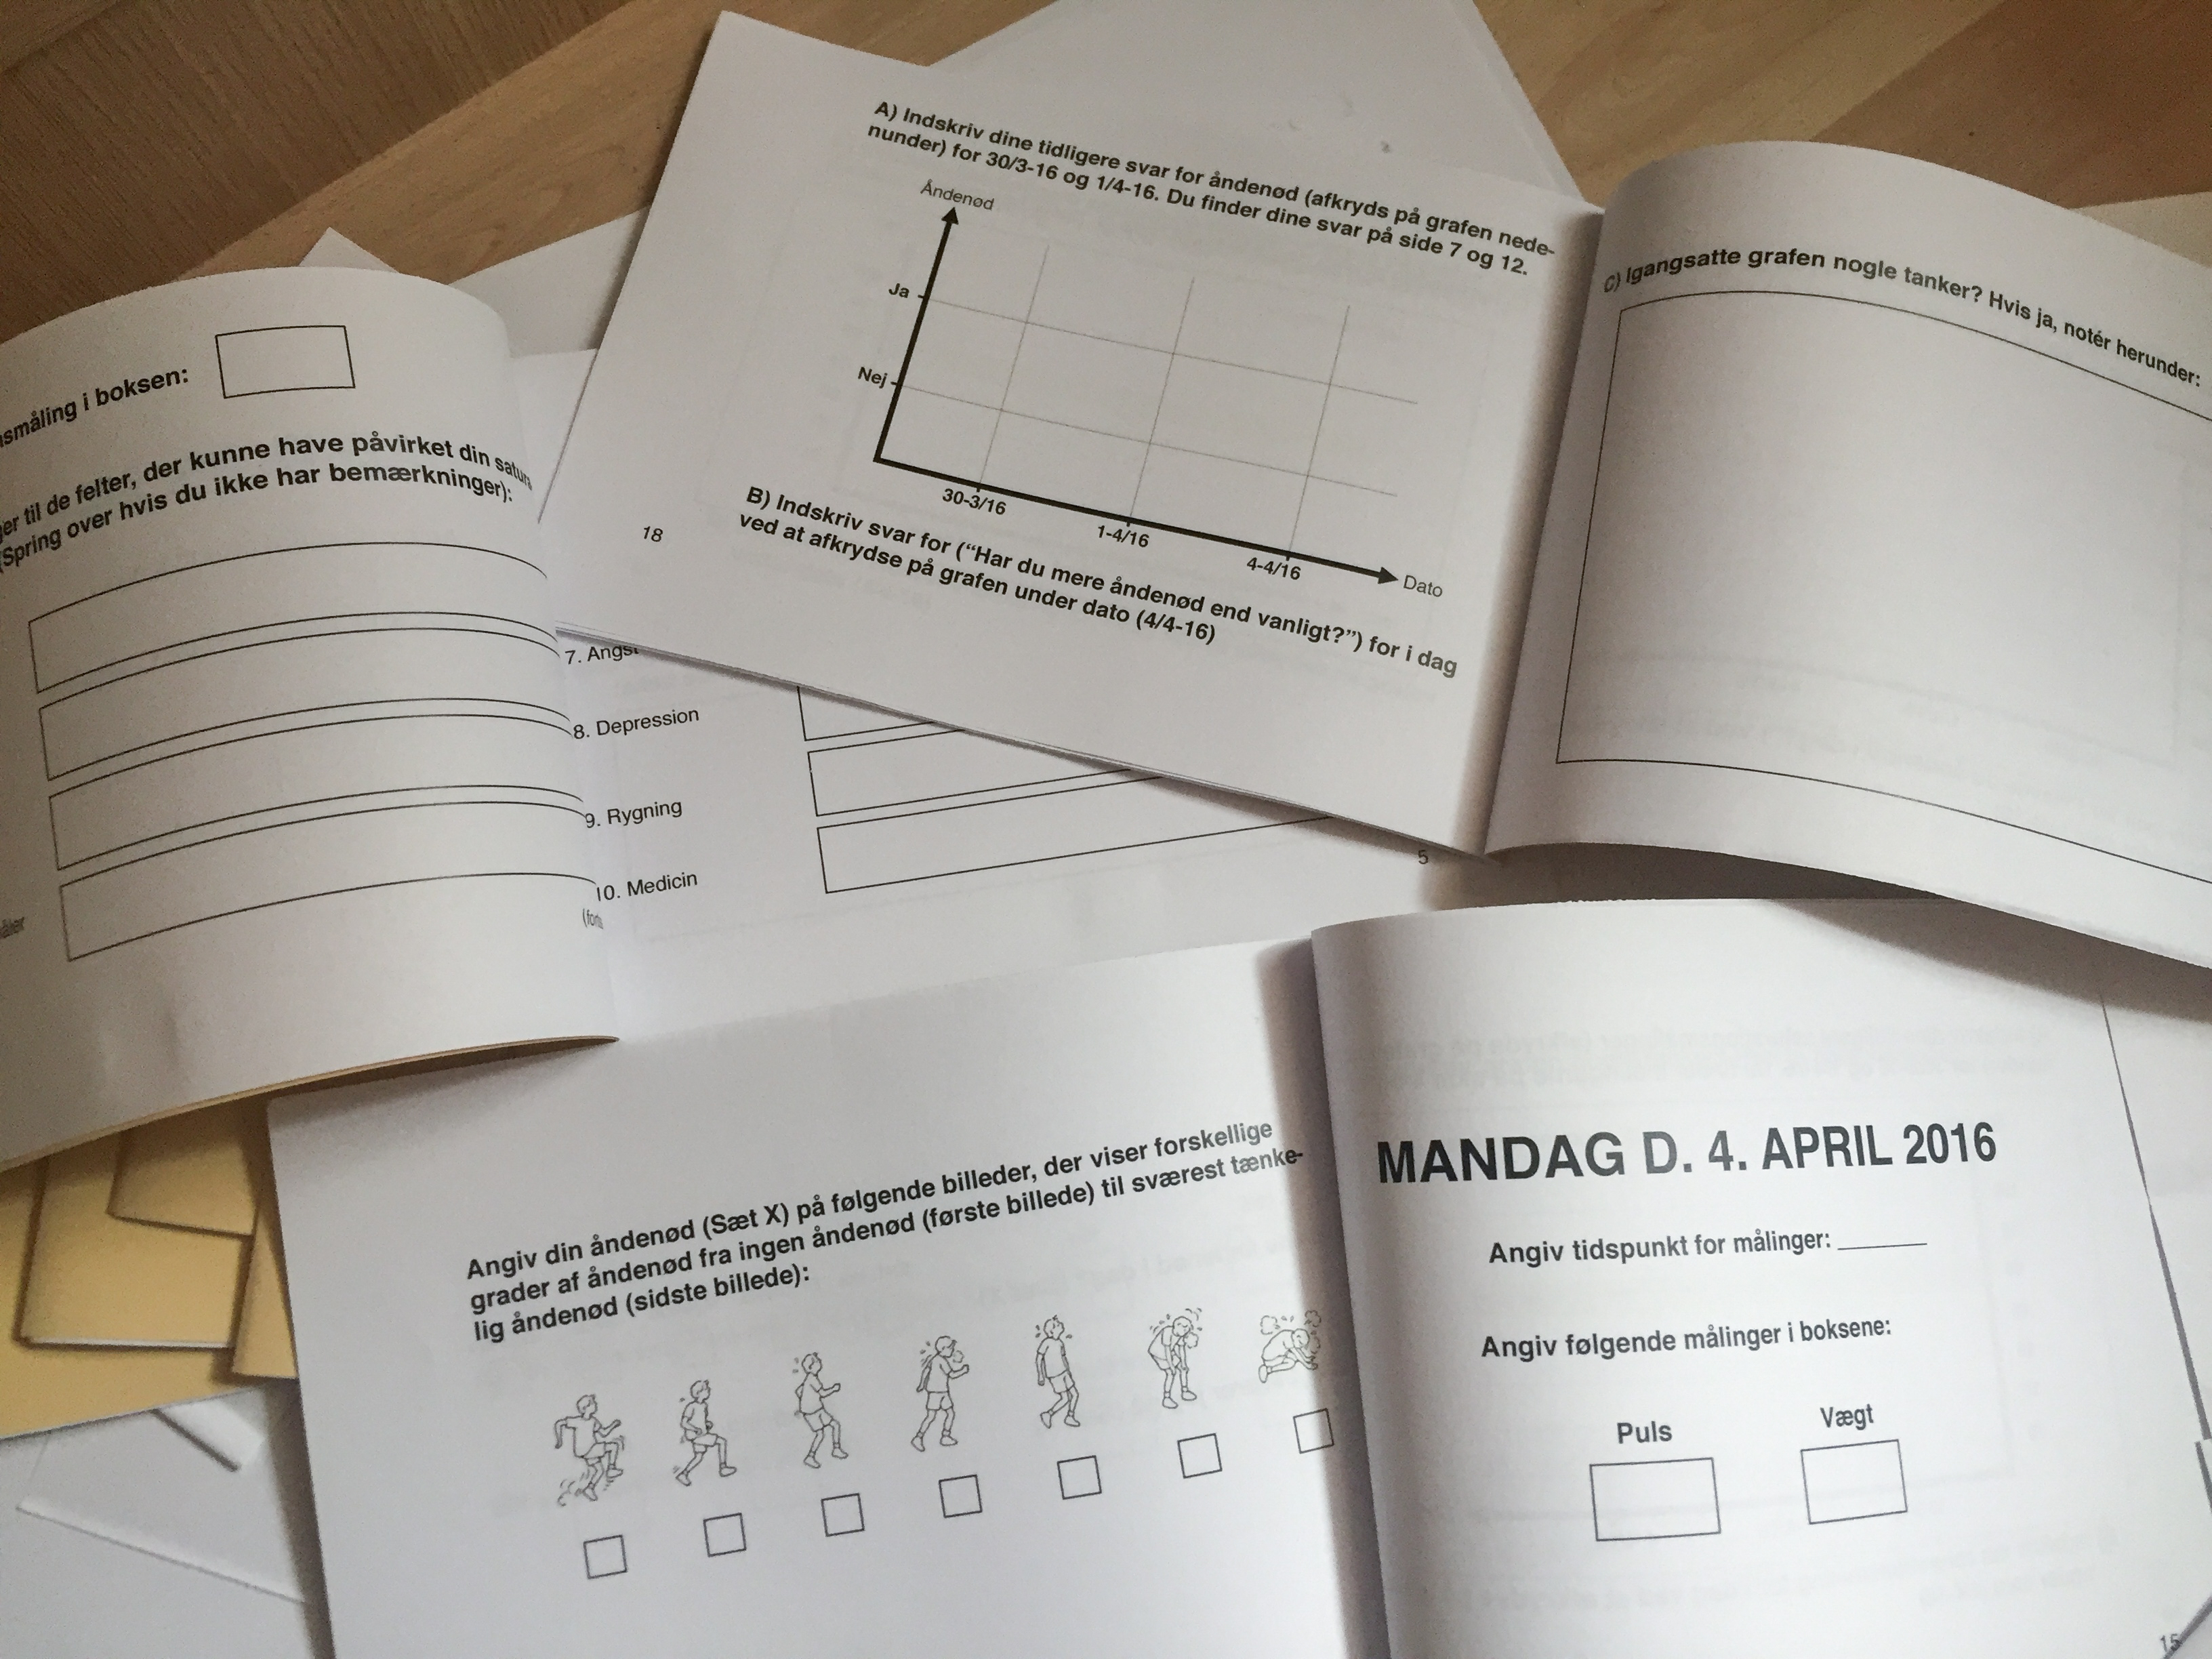
\includegraphics[width=\textwidth]{img/workbook2}
   %\caption{Flower two.}
 \end{minipage}
  \caption{Workbooks with assignments}\label{fig:workbook}
\end{figure}


In Study 1, patients expressed difficulties rating symptoms subjectively, due to lack of baseline understanding and low granularity of answer options. Patients had to reflect on a time series graph of previous measures (showing baseline) while entering current measure in one assignment. In another assignment, patients assessed dyspnea on different scales: (1) Relative to usual baseline (binary), (2) absolute (five-point scale inspired by the questionnaire-items in EXACT PRO \cite{exact}) and (3) using visuals (Dalhousie Pictorial Scale \cite{dalhousie}). 

Finally, patient had to reflect on a time series graph of previous oxygen saturation measures (long-term reflection). A recommended level (also referred to as goal or "normal area") was marked on the graph to trigger reflection on a potential mismatch in accordance with Festinger's cognitive dissonance theory \cite{Rivera}.

\begin{figure*}
 \centering
 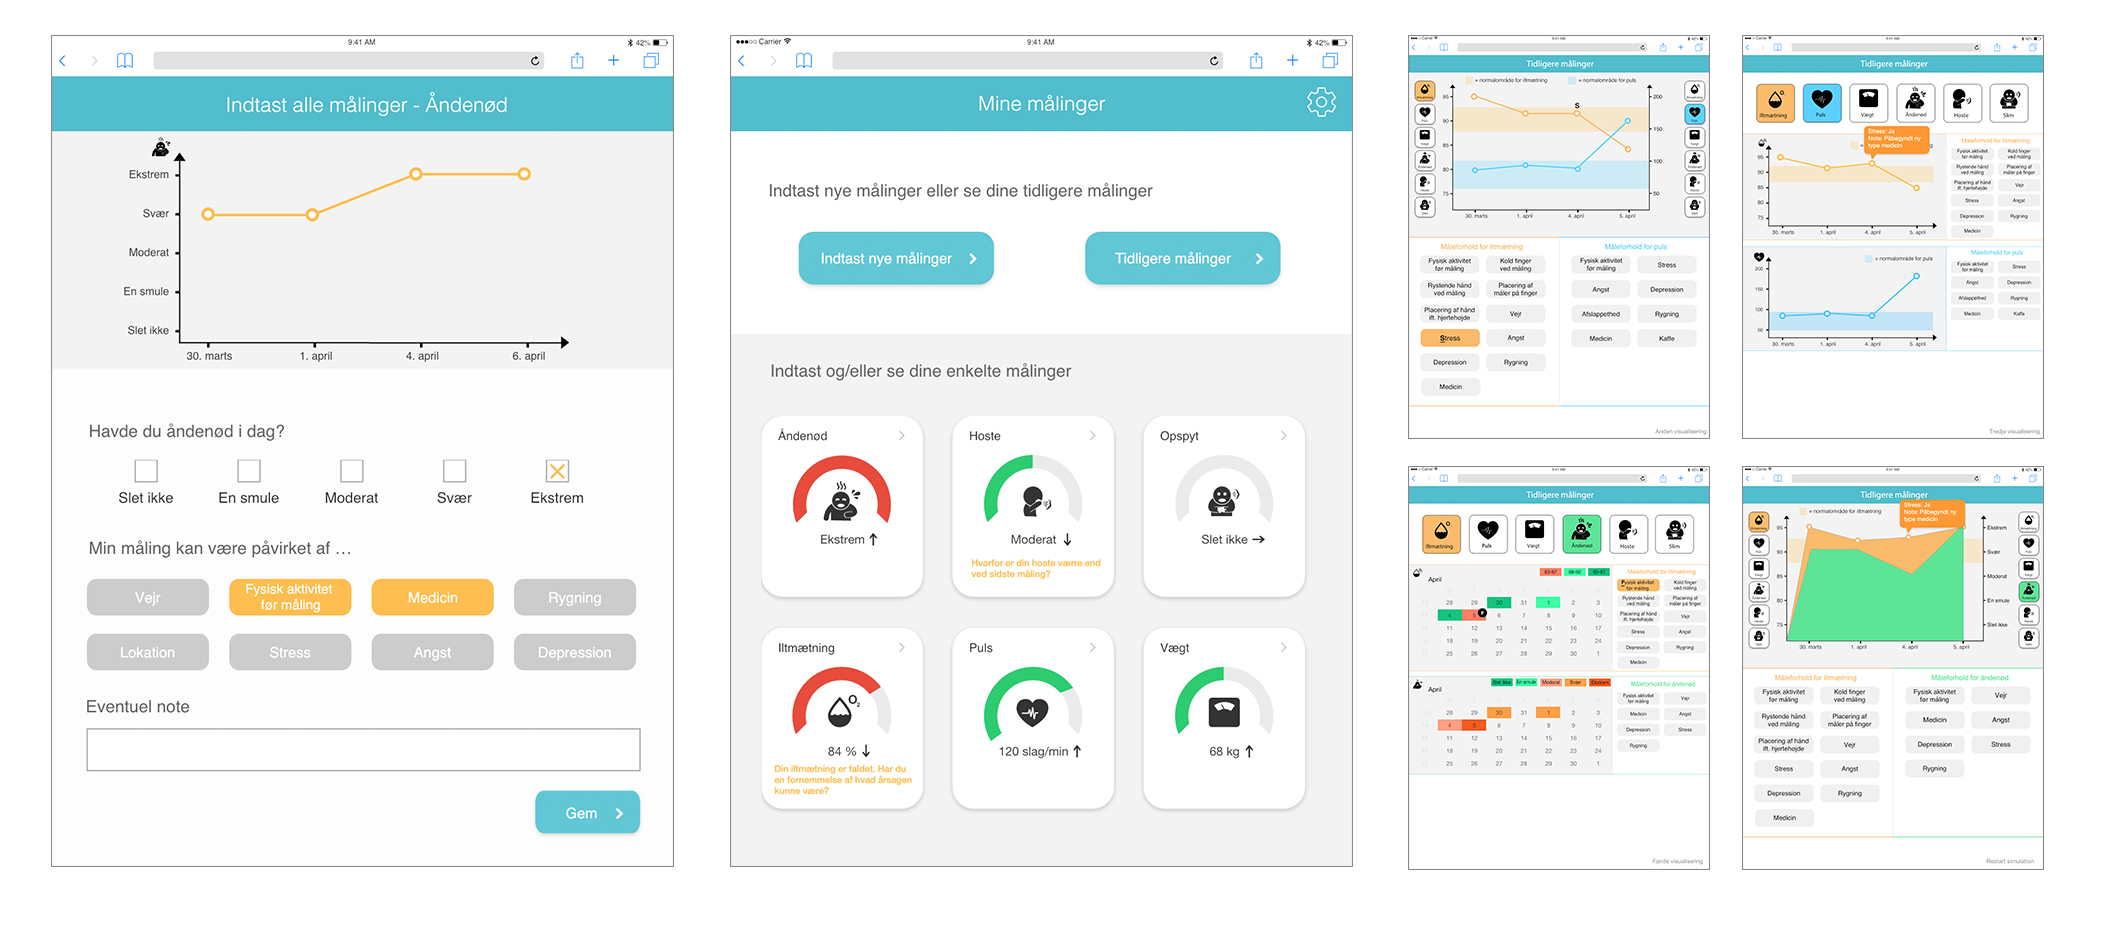
\includegraphics[width=2.1\columnwidth]{img/screens}
 \caption{Screens from the prototype: Collection page (left), Dashboard (middle), Four visualizations of history data (right): V1 (top left), V2 (top right), V3 (bottom left) and V4 (bottom right)}~\label{fig:design}
\end{figure*}

\subsection{Prototype Design}
\subsubsection{Improving Reliability and Validity of Measures}
The collection page had features similar to the workbook assignments (See Figure \ref{fig:design}). A time series graph visualising patients' previous measures supported patients in remembering previous events while entering data in the prototype. Symptom rating options were scale-based instead of binary as patients were used to, inspired by questionnaire-items in EXACT-PRO \cite{exact}. We further introduced the option to toggle context-relevant variables for each measure in the prototype to provide enrichment \cite{Rivera}, support reflection while collecting and later review (description follow in next section).

\subsubsection{Supporting Short-term and Long-term Reflection}
From literature, we found that supporting both short-term and long-term reflection can be important, depending on the conditions in which the user might self-track \cite{Li2010, Muller}.

To support short-term reflection, we provided patients with a dashboard view after collection (See Figure \ref{fig:design}). The dashboard view aimed at allowing patients to reflect on current status immediately after collection and increase awareness on their current status \cite{Cuttone, Muller}. We included reflective questions to trigger reflective description (R1) or higher levels of reflection on this view and to encourage users to further explore their data \cite{Fleck, Muller}. E.g. \textit{"Why are you coughing more than last time you measured?"}. Gauges for each measure showed current measure in relation to the recommended level and arrows indicated change from previous measure (day-to-day variations). The system used color indications (red, yellow and green), where red or yellow highlighted a potential mismatch and thereby aimed at actively triggering reflection in accordance with Festinger's cognitive dissonance theory \cite{Rivera}. 

To support long-term reflection, we designed four different visualisations (See Figure \ref{fig:design}). (V1) Time series graphs with option to compare two measures, (V2) Time series graphs stacked vertically, (V3) Calendar heatmap and (V4) Area graphs with option to compare two measures. V1, V2 and V4 were proposed to foster reflection on upwards and downwards trends or symptoms deviations to increase awareness on a worsening in condition \cite{Rivera}. V1 and V5 differed in that they allowed for comparison of multiple measures that could trigger reflection on, how measures were related or changed over time \cite{Cuttone}, affording dialogic reflection (R2) \cite{Fleck}. Recommended levels were highlighted on all four visualisations to increase awareness on discrepancies \cite{Li2010} and trigger reflection. V3 was proposed as an alternative to time series graphs as mentioned by Cuttone et al. to support reflection on periodic patterns using color shades to indicate deviations from recommended level \cite{Cuttone, Li2010}.  

To further support long-term reflection, we provided the option to toggle on discrete events on the visualisations (context-relevant variables) \cite{Sorensen}. This feature was included to support reflective description (R1) and dialogic reflection (R2) by allowing for exploration of relationships between context-relevant variables and measures otherwise invisible \cite{Fleck}.  

\subsection{Participants and Method}
We asked the same patients as in Study 1 to participate in feedback sessions on the redesigned system. All patients and three spouses (P2S, P5S and P6S) participated, except P4 who was hospitalized. Feedback sessions were held in the patient's home and audio-recorded. Sessions lasted approximately one hour. 

Patients completed workbook assignments three days a week (Monday, Wednesday and Friday) delivered one week prior to the feedback sessions. Feedback session were divided into a workbook session and a prototype session, where two researchers were present. One researcher took the facilitation role and asked patients follow-up questions emerged from Study 1, while the other researcher went through the workbooks and prepared for the workbook session. After the follow-up, the researchers shifted roles. The researcher responsible for the workbook interviewed patients and discussed assignments, while the other researcher prepared the prototype. The prototype preparation involved adjusting the prototype to use patient's own values for visualisations (collected in workbooks) to encourage reflection on patients' own experiences rather than fictive values. In the prototype session, patients went through each screen in the prototype and completed usability tasks and discussed understanding and thoughts on the prototype. The researcher encouraged both patients and their spouses to think-aloud and provide their points of view. 

\subsection{Results}    
We identified two types of patients in this study: Active and Passive. Passive patients (P1 and P3) took the role as data providers and did not see any benefits in neither short-term or long-term reflection provided by the system. Active patients (P2 and P5) were more open-minded towards engaging in the discussion of reflecting on self-tracked data. 

\subsubsection{Reliability and Validity of Measures}
Not all patients were consistent in terms of \textit{when} and \textit{how} they took measures. Some patients had specific routines (e.g. always before breakfast), while others were not consistent (e.g. P1 only weighed himself every three weeks). 

Passive patients and P6S lacked knowledge on relevance of context and how some of the provided context variables influence their measures. E.g. P1 and P6S questioned whether and why a cold finger when taking oxygen saturation measures had an influence. Active patients ensured taking measures under comparable conditions. Patients mentioned additional context variables relevant for their measures (e.g. mood, talk, supplemental oxygen). P2 and P6S specifically asked for guidelines on taking measures. \textit{"For some measures, an explanation would be good. For example do not take measure if this and that"} (P6S).

All patients preferred higher granularity options when rating symptoms more than binary. P5 and P6 mentioned that they preferred higher granularity, because it made it possible to show degrees. \textit{"How much is a no? If we say yes or no to the hospital, they still do not know what we are thinking .. then they'll call us and we'll have to explain it is severe"} (P6S).

Asking to rate symptoms without a baseline comparison (\textit{"Did you feel breathless today?"}) and having five answering options (not at all, slightly, moderately, severely, extremely) or visuals as options caused difficulties for some patients, because they experienced several of the options during the day. \textit{"I have been through all of the provided options that day. How do you want me to answer that?"} (P5). Patients further had different perceptions of what usual is, when asked to rate relative to usual baseline. \textit{"(..) I base that on when I'm at my best"} (P3), \textit{"usual is when it is an ordinary day"} (P5) and \textit{"If she is not more breathless than yesterday, then we'll just submit a no"} (P6S).

Patients presumed that it would not be of benefit to them to have a time series graph showing their baseline while collecting. "\textit{I do not think it has any effect to see a graph}" (P3). P2 mentioned, "\textit{I shouldn't answer based on what I answered last time. I should answer what it is now and here}".

\subsubsection{Short-term and Long-term Reflection}
In the prototype session, some patients were not willing to reflect on visualisations of current status, reflective questions or history data. E.g. \textit{"I do not care what my status is.. I just submit data.. do not walk around and think everyday .. I know how I am feeling"} (P3). P5 expressed interest in current status and what action should be taken, \textit{"I'm more concrete. Where am I right now and what can I do about it?"} (P5). The dashboard view helped some patients in getting an quick overview of their health status (e.g. P5). P2 mentioned that the arrows helped him \textit{"quickly see if it [a measure] is going up or down"}. Reflective questions were not noticed by the patients. In passive patients reflective questions did not trigger any reflection (R0), while active patients proposed lower level explanations as answers (R1), when we prompted them to answer the question in the system. E.g. to the question \textit{"Why are you coughing more than last time you measured?"}, P5 answered: \textit{"Right now it is likely because I talk too much"}.

None of the patients expressed interest or benefits in having access to previous measures prior to the feedback session, e.g. \textit{"I do not need it [access to history data]"} (P3). Several patients relied on the healthcare monitoring \textit{"I have a nurse who is good at keeping an eye on me"} (P5), \textit{"I do not need it [access to history data]. If it [measure] is too low, they call and ask me why"} (P1). P2 similarly expressed that he did not have the necessary knowledge to find it useful \textit{"I do now know what they use it for, the scales they use and the language.. I do not understand it. I count on them reacting if there is anything"} (P2).

Providing patients with a recommended level that they could compare their measures against, provoked negative feelings among some: \textit{"I prefer not to be told in the morning that I'm gonna get an awful day"} (P5), \textit{"It's ok if it's just a single measure, but if it is constant, I would start thinking.. It's going fast now"} (P2). While P5 mentioned that she would ignore the recommended level, because it did not match with her own goal, \textit{"I thought, you can forget it [about provider-recommended level]. I'll just do what I usually do"}, P2 suggested that he would strive to keep his measures within the recommended level, \textit{"then it's not that bad if I keep it above that [lower threshold]"}. P6S indicated that if his wife's oxygen saturation was above normal area, he would start wonder whether the oxygen supply was set too high and initiate action. \textit{"If it starts to go over here [below normal area], we have to do something"} (P6S).

Despite none of the patients initially expressed benefits in having access to history data, two patients (P2 and P5) changed their attitude after the prototype session. \textit{"This gives more information about me (...) it's nice to be able to go back.. Is it better than 14 days ago?"} (P2). One patient mentioned needing a purpose and time to reflect for gaining any benefits from history data, in accordance with Fleck \& Fitzpatrick \cite{Fleck}: \textit{"There might be days where I sit with it and have an idea about what I'm looking for, which might trigger some thoughts"} (P5). Others were more reluctant on reflecting on history data. P3 did not see any benefits and found it troublesome, while P1 did not think it was his job to look at history data, \textit{"this is only for people who has to sit and analyse the numbers"} (P1). 

V1 afforded finding relations between measures e.g. by comparing, \textit{"you can have them (measures) together and see how they affect one another"} (P2). V3 was more attractive to others, who found it more concrete and provided a quick overview, \textit{"it (V3) is the one I get the quickest.. If you are in doubt what the colors mean, you can see them down there"} (P5). PS6 thought that he would start with V2 and then use V1 after becoming more advanced. 

Assignments in the workbook and prototype elicited only limited findings on patients' reflective thoughts on the design proposals. While we did use patients' own values rather than fictive values to discuss the workbook and prototype assignments in terms of long-term reflection, we used fictive values on the dashboard, which could have been a barrier for reflection in some patients. Additionally, patients might have found it difficult to reflect, because (1) the interview period was time-limited and (2) a reason (e.g. a worsening in health status) was needed to trigger reflection. Taking into account the findings from this study, we decided to implement the system with a few adjustments and evaluate it on other COPD patients in a two weeks trial. 